\pagestyle{fancy}
\rhead{\bfseries OCR A-Level Computer Science}
\chead{\mdseries \thepage}
\lhead{\bfseries Jonathan Kasongo \mdseries — May 2025/26}
\lfoot{\sffamily Candidate number: N/A}
\rfoot{\sffamily Centre number: N/A}

\chapter{Development}
\label{chap:development}

% Provided evidence of each stage of the iterative
% development process for a coded solution
% relating this to the break down of the problem
% from the analysis stage and explaining what they
% did and justifying why.

% Well structured and modular, code annotated, DRY

% Validation evidence 

\section{Development overview and sub-tasks}

We apply the principle of decomposition to our development
plan by splitting up the development of the system into 
a number of smaller sub-tasks. Each sub-task relates to it's
relevant circled number in our problem breakdown (see section 
\ref{sec:breakdown}).\\ \vspace{0.2cm}

In doing this we \textbf{clearly} relate each iteration
to a part of the problem breakdown.\\ \vspace{0.2cm}

\begin{longtblr}[
  caption={Development sub-tasks.}
]{
  colspec={cX}, row{1}={lightestgray}
}
  Number & Sub-task \\
  \circled{1} & Design home page \\
  \circled{1.1} & Design help page \\
  \circled{1.2} & Design login page \\
  \circled{1.3} & Document the backend code throughout\\
  \circled{2} & Allow users to create their account\\
  \circled{3} & Implement login system with password resets \\
  \ldots & \ldots \\
  \circled{A} & Deploy website \\
\end{longtblr}
\vspace{0.2cm}

Finally note that all the code for this project is open source
and freely available for you to view on github:
\url{https://github.com/zzzNathan/Video-Conferencer}. \\ \vspace{0.2cm}

\textit{We may shorten code snippets using ellipsis though the
entire code at such point in development is available by finding the 
correct commit on Github. This commit number as well a link are both
provided at the end of each iteration.}

\section{Iteration 1}

% explaining what they did and justifying why

During this iteration I wanted to finish up designs for a few 
of the pages that will appear on our website. This should 
clear up sub-task \circled{1} and \circled{1.2}.

\subsubsection{Home page}

\begin{figure}[H]
\centering

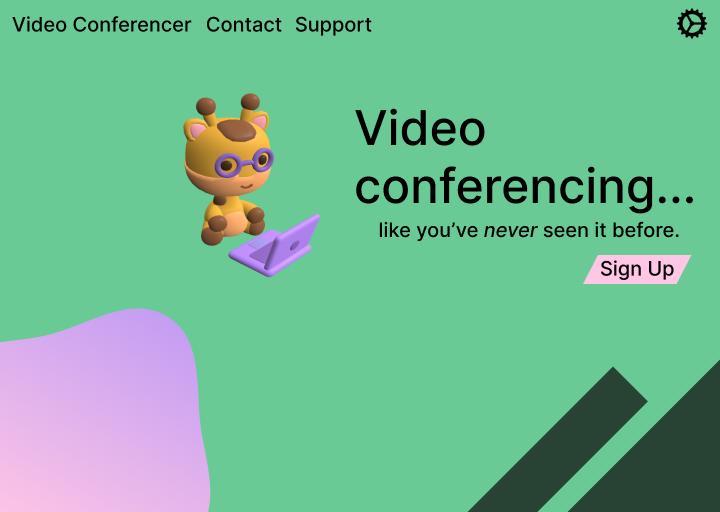
\includegraphics[scale=0.2]{Images/HomeUI_2.png}

\caption{2nd Mock up of the home page.}
\label{fig:ui2}
\end{figure}

\begin{figure}[H]
\centering

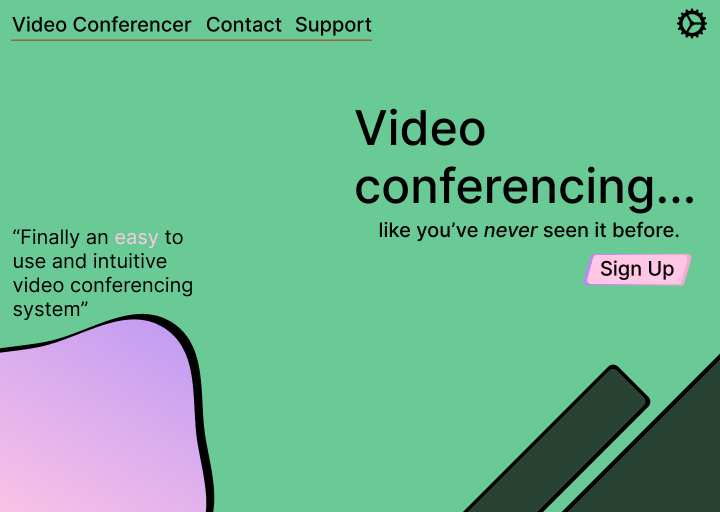
\includegraphics[scale=0.2]{Images/HomeUI_3.png}

\caption{3rd Mock up of the home page.}
\label{fig:ui3}
\end{figure}

\textit{Description:}
I started by cleaning up the mock design for our home page.
The first mock up was a very basic outline for how I wanted to 
style the page, so in the next couple iterations I polished 
the design and added more designs to fill the web page. These
additions made the home page feel more complete and less 
bare-bones, consequently making the webpage feel more 
professional for the user. \\ \vspace{0.2cm}

\textit{Explanation and justification:}
I created mock ups of the home page and all other web pages 
before actually coding them up. Designing mock ups helped 
to give me a sense of direction in the process of creating a 
webpage design in HTML and CSS. If I were to try to create 
the design on the fly whilst writing code I would have no
reference to use and my design would end up being lackluster 
and poorly thought out. By purely focusing on the page layout 
and design first, I can create a page that I am happy with in 
Figma and then focus on converting this design into HTML and 
CSS code using my mock ups as a reference as to what the end 
product should look like. Indeed by starting with designing 
mock ups, it gives me something to aim for when writing up 
the code to produce our home page. Then by iteratively
improving upon the design mock ups I created I enhance
the look of the final home page design, in turn creating
a superior user experience.
\\ \vspace{0.2cm}

\textit{Description:}
I transfer my designs into HTML and CSS. However after some 
reseach I come to the conclusion that I'd prefer to write 
sass and compile this into CSS instead, because of it's 
superior syntax. \\ \vspace{0.2cm}

\textit{Explanation and justification:}
The next step was to transfer this design into HTML and CSS. 
Since my designs made use of a collection of frequently used 
colours I concluded that it would be useful to be able to use
these colours as defined variables instead of having to write 
out their hex colour codes each time 
(see section \ref{sec:ui}). However the native CSS syntax 
looks something like this. (Taken from \url{https://www.w3schools.com/css/css3_variables.asp})

\begin{minted}[linenos, bgcolor=lightestgray]{css}
:root {
  --blue: #1e90ff;
  --white: #ffffff;
}
\end{minted}

I personally found this syntax particularly disgusting, 
after doing some research I came across this stack overflow 
answer \url{https://stackoverflow.com/a/1877358}. After digging
into exactly what "sass" and "less" were I decided to use sass
as an extension of my CSS because I liked the look of it's 
syntax better. Sass (\textbf{S}yntactically \textbf{A}wesome 
\textbf{S}tylesheet) is a CSS extension language that 
provides a new syntax for writing CSS as well as a number of 
features that prevent repetition in the code like variables, 
functions and more. The sass code is saved in a \texttt{.sass}
file then one can compile the sass code into CSS by using the
command \texttt{sass <sass file name> <output css file name>}.
\\ \vspace{0.2cm}

After blocking in the basic elements of our webpage the HTML 
and sass code looked like this.

\subsubsection{Prototype 1}

\underline{main.html}

\begin{minted}[linenos, bgcolor=lightestgray]{html}
<!DOCTYPE html>
<html>

<head>
  <meta charset="UTF-8">
  <meta name="viewport" content="width=device-width, initial-scale=1.0">
  <link href='https://fonts.googleapis.com/css?family=Inter' rel='stylesheet'>
  <link rel="stylesheet" href="styles.css">
  <title>Video-Conferencer</title>
</head>

<body>
  <div class="Headlines">

    <div class="Main_Headline">
      Video conferencing...
    </div>

    <div class="Sub_Headline">
      like you've never seen before.
    </div>

  </div>
</body>

</html>
\end{minted}

\underline{styles.sass}

\begin{minted}[linenos, bgcolor=lightestgray]{sass}
// Colour definitions
$Col_Main:       #69ca95
$Col_Secondary:  #284333
$Col_Tertiary:   #9a6442
$Col_Accent:     #ffc6e5
$Col_AccentDark: #c49df2

// Setting font and background colour
body
  background-color: $Col_Main
  font-family:      'Inter', sans-serif

// Styling for the main headline
.Main_Headline
  width:       701px
  height:      238px
  font-size:   96px
  ... 

// Styling for the sub headline
.Sub_Headline
  width:       603px
  height:      101px
  font-weight: 500
  ...
\end{minted}

This code produced our 1st prototype.

\begin{figure}[H]
\centering

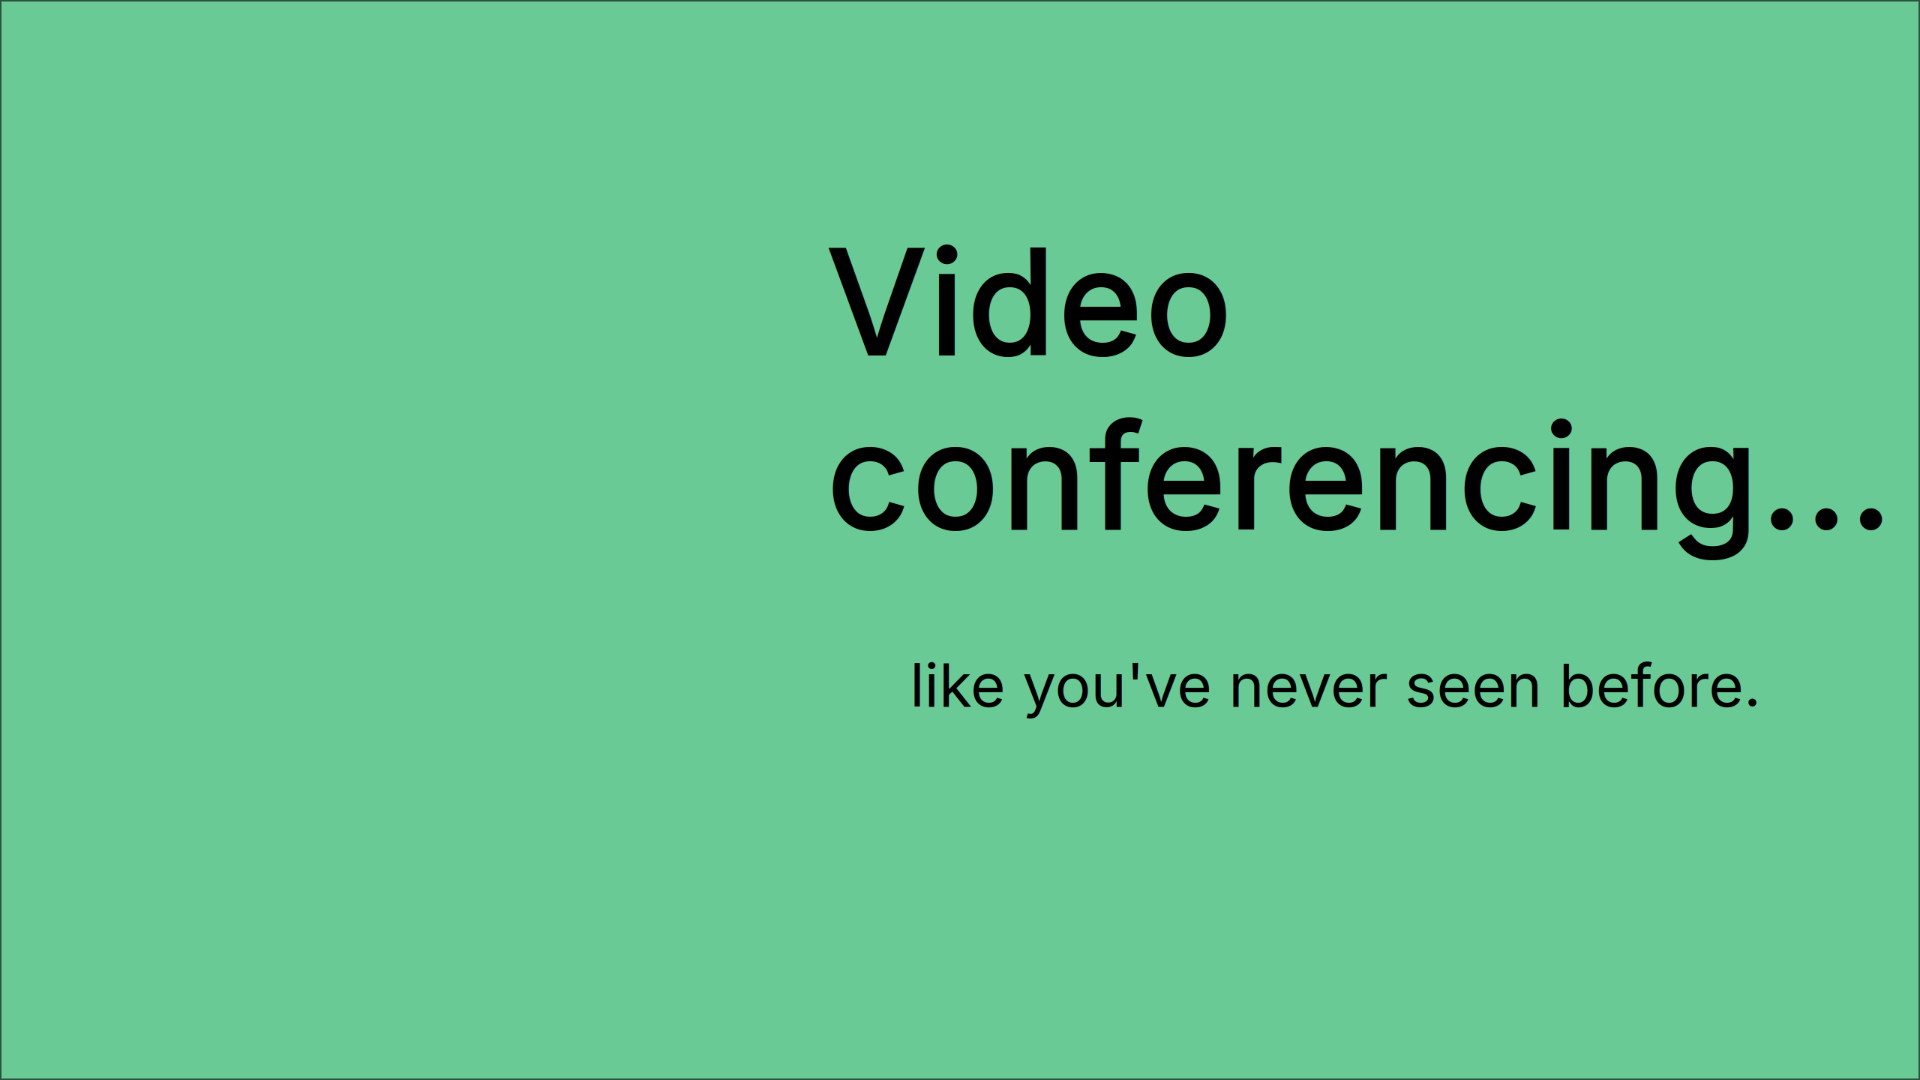
\includegraphics[scale=0.2]{Images/Proto_home1.png}

\caption{Home page prototype 1}
\end{figure}

{\color{gray} \hrulefill} \\ \vspace{0.2cm}

{\sffamily Client Feedback:} 
\begin{itemize}
  \item The headline and sub-headline are too far apart.
  \item The main headline takes up too much space on the page.
  \item The "never" isn't italicised.
\end{itemize}

{\color{gray} \hrulefill} 

\subsubsection{Prototype 2}

\textit{Description:} 
I pivot to using vector graphics in order to position the 
elements on our webpage. \\ \vspace{0.2cm}

\textit{Explanation and justification:}
After writing the code for the first prototype I soon realised
that actually writing the text for the main headlines and 
manually positioning it would be a very tedious task. So I 
decided to instead export the headline as well as the graphic 
designs as \texttt{.svg} files from Figma. This means I
wouldn't have to worry about carefully positioning and spacing
the headlines individually and I could instead just position 
them as 1 vector image. The \texttt{.svg} image format was 
chosen because vector images never lose their resolution even
when scaled, you will still be able to see clean and crisp 
images no matter how much you zoom in, something which isn't
achievable with the \texttt{.jpg} or the \texttt{.png} formats.
In the rare case that \texttt{.svg} files are not supported
for the user's browser \footnote{Vector images are supported
by all browser except Internet Explorer 8 and below, and 
Android 2.3 browser and below.} we also provide fallback 
\texttt{.png} image files for these users. This ensures that 
users will be able to see the page's content no matter their 
choice of browser, hence improving the robustness of our
system.\\ \vspace{0.2cm}

Our code now looks like this.

\underline{main.html}
\begin{minted}[linenos, bgcolor=lightestgray]{html}
...

<body>

  <div id="Headline_container">
    <object id="Headline" data="Images/Headline_text.svg" type="image/svg+xml">
      <img src="Images/Headline_text.png">
    </object>

    <object id="Sign_up" data="Images/Sign_up.svg" type="image/svg+xml">
      <img src="Images/Sign_up.png">
    </object>
  </div>

  <div id="Bot_left_graphic_container">
    <object id="Bot_left_graphic" data="Images/Bot_left_graphic.svg" type="image/svg+xml">
      <img src="Images/Bot_left_graphic.png">
    </object>
  </div>

  <div id="Bot_right_graphic_container">
    <object id="Bot_right_graphic" data="Images/Bot_right_graphic.svg" type="image/svg+xml">
      <img src="Images/Bot_right_graphic.png">
    </object>
  </div>

</body>

</html>
\end{minted}

\underline{styles.sass}
\begin{minted}[linenos, bgcolor=lightestgray]{sass}
... 

// Setting font and background colour
body
  height:           100vh
  margin:           0
  background-color: $Col_Main
  ...

// Positioning the headline svg
#Headline_container
  position: relative
  top:      10%
  left:     45%

// Positioning the signup svg
#Sign_up
  position: absolute
  top:      75%
  left:     35%

// Positioning the bottom left graphic svg
#Bot_left_graphic_container
  position: relative
  top:      0%

// Positioning the bottom right graphic svg
#Bot_right_graphic_container
  position: relative
  left:     50%
  bottom:   75%
\end{minted}

This code produced our 2nd prototype.

\begin{figure}[H]
\centering

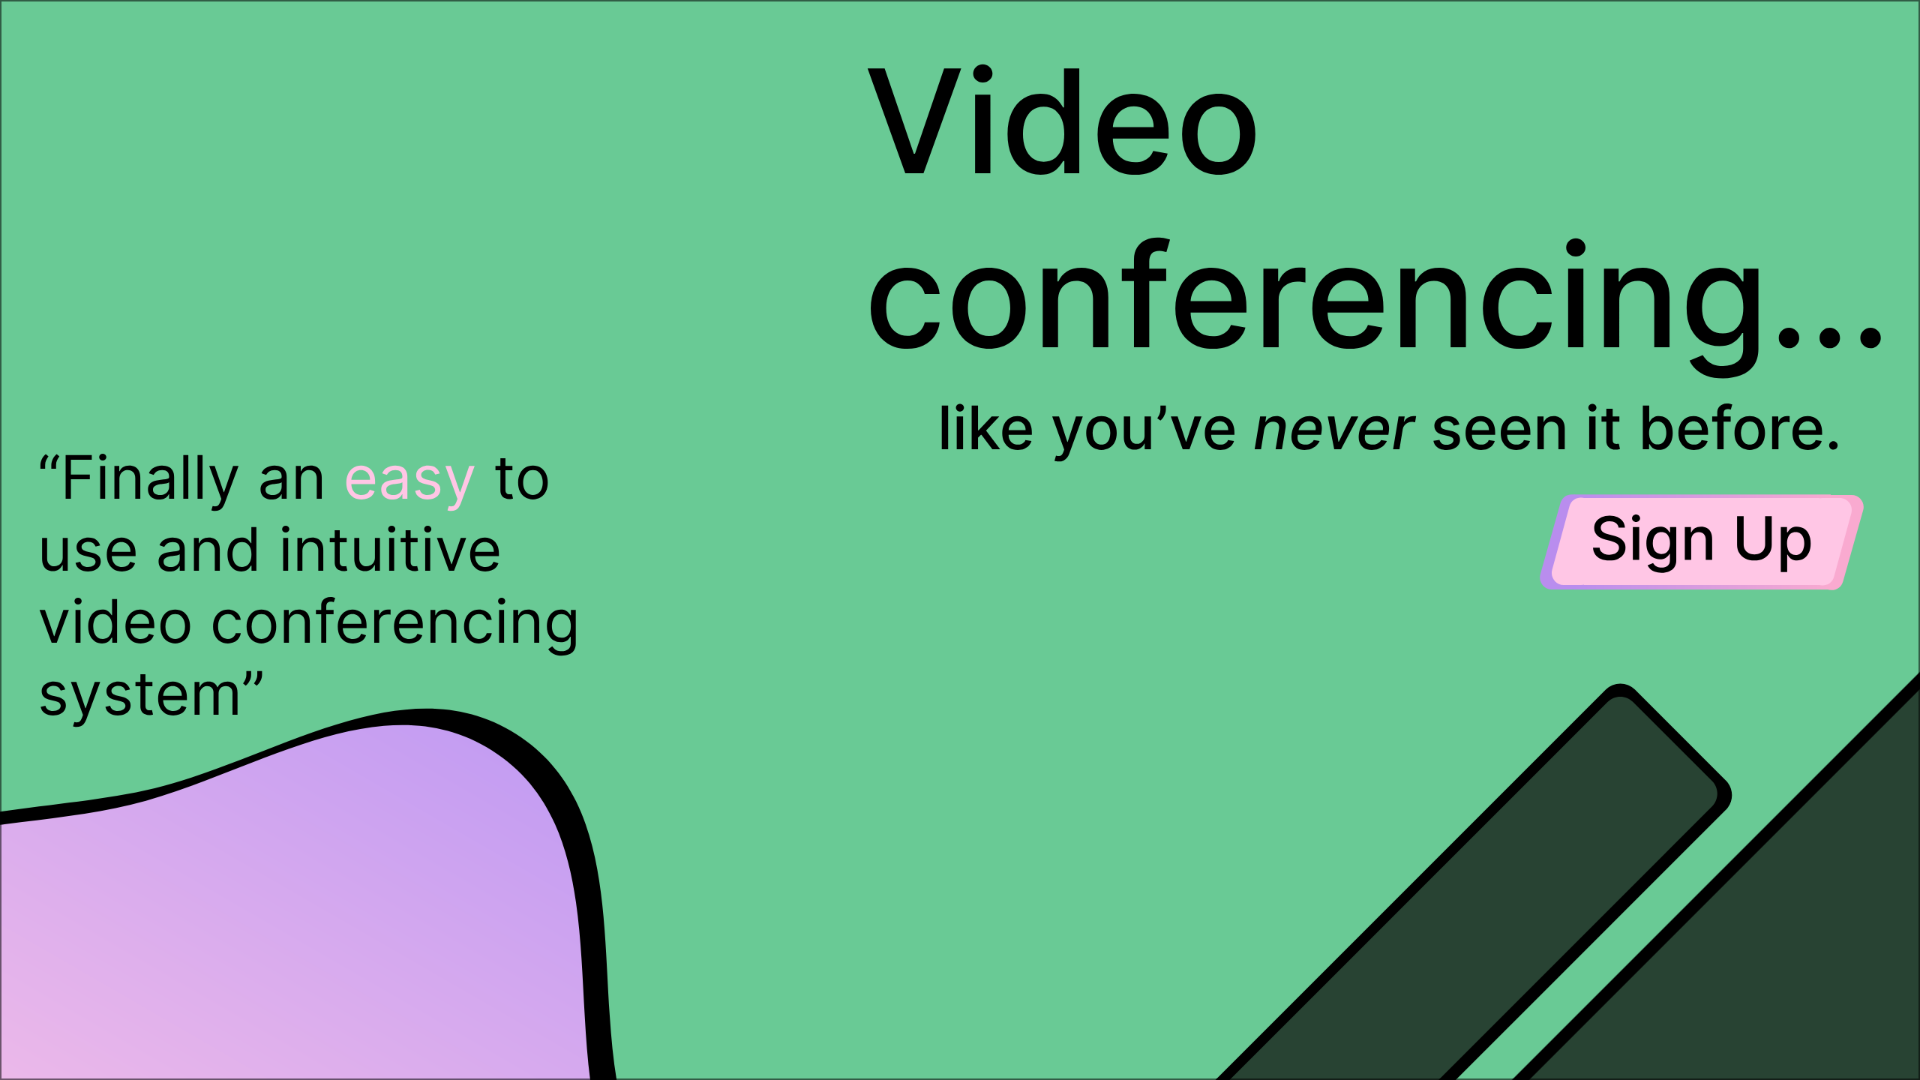
\includegraphics[scale=0.2]{Images/Proto_home2.png}

\caption{Home page prototype 2}
\end{figure}

{\color{gray} \hrulefill} \vspace{0.2cm}

{\sffamily Client feedback:}

\begin{itemize}
  \item We are still lacking a navigation bar at the top.
  \item All the elements feel as though they take up too much space on the page.
\end{itemize}

{\color{gray} \hrulefill} 

\subsubsection{Prototype 3}

\textit{Description:}
I redesign the entire look and aesthetic of our system.
\\ \vspace{0.2cm}

\textit{Explanation and justification:}
After reviewing the design holistically, I felt that I could 
have done a better job designing the page to contribute to 
creating a professional looking system, so I re-did my 
designs in Figma. The graphic designs on our previous 
prototype designs were nice but they felt "too much",
so I decided I should tone back the designs and focus on 
simplicity. Indeed our target user base is comprised of 
elderly ones who might not appreciate such a bright and 
vibrant design, the design would have not only been 
overwhelming for the average user but also would have made 
our system seem unprofessional and childish. This is seen 
in the complete lack of cohesion between the various graphics 
on that page. The dark green triangle graphic creates an 
unwanted contrast between it and the rest of the page to the 
point that it becomes the centre of attention and one of the 
first things that will catch the user's eye.
Furthermore the choice for the background colour
was too bright and vibrant and didn't allow other elements 
to stand out as much as they should.\\ \vspace{0.2cm}

In designing the revised 
prototype I took inspiration from the design of the 
Zen browser home-page \url{https://zen-browser.app/}. They 
simply have a navigation bar, a main and sub headline, a call
to action button and some testimonials along the bottom. Here
is the newest design. (Of course after making such significant
changes I contacted my client and asked for permission to
change to this new design and he agreed). \\

\begin{figure}[H]
\centering

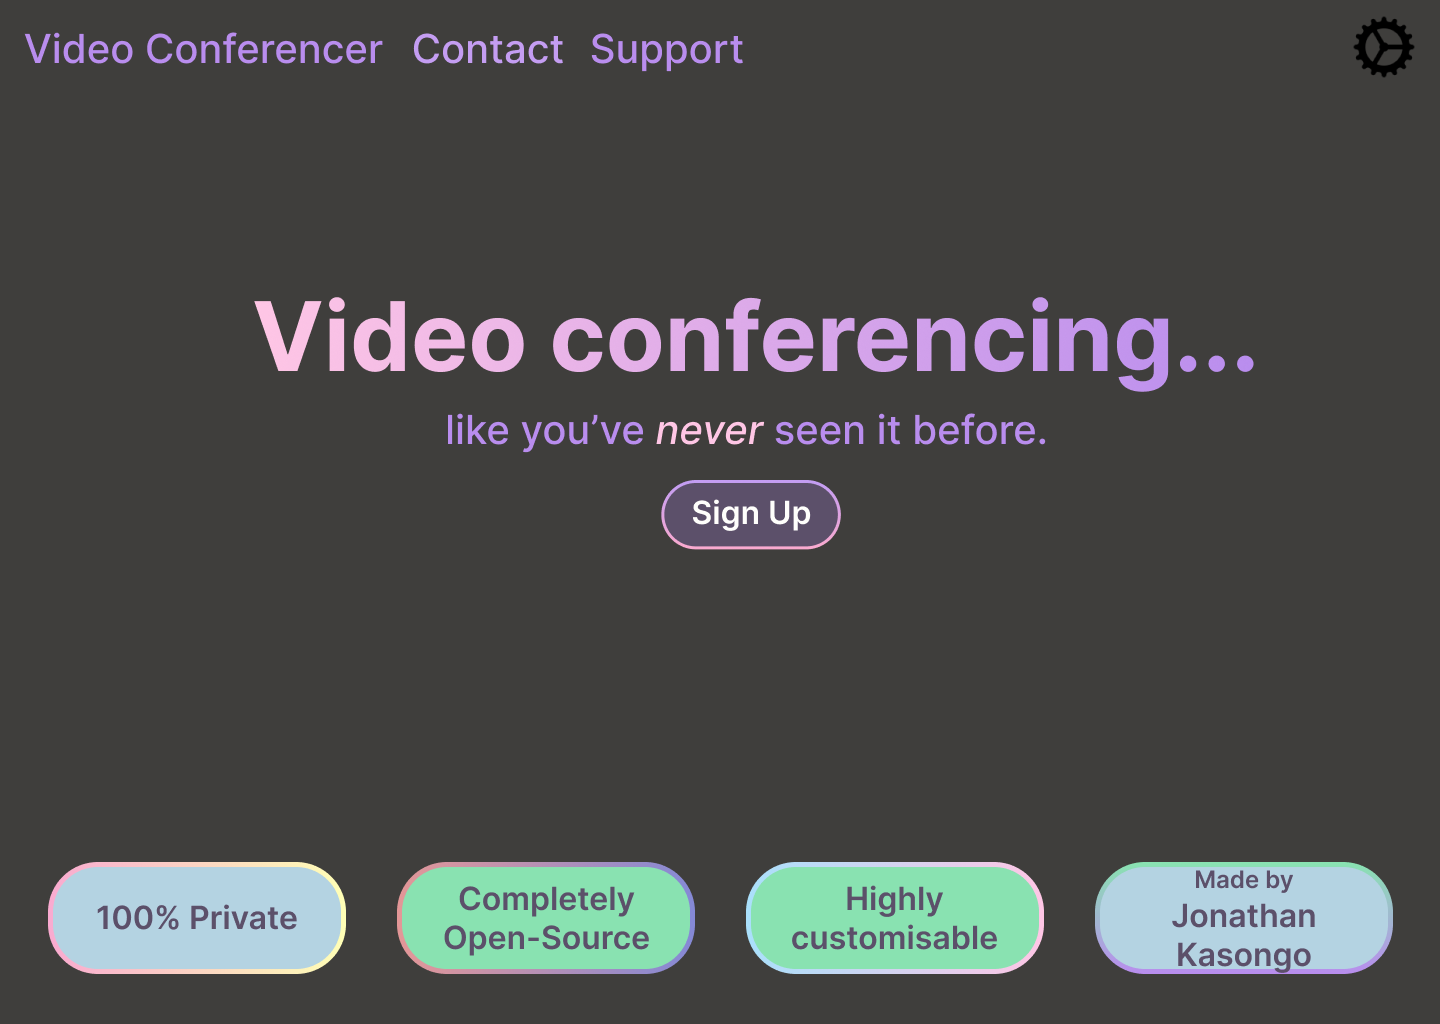
\includegraphics[scale=0.2]{Images/HomeUI_4.png}

\caption{4th Mock up of the home page.}
\end{figure}

Now in relation to the point \textit{"the elements feel as
though they take up too much space on the page"} I found that 
an appropriate solution was to simply scale every element on 
our page to 75\%. This then made the page look closer to the
one design in Figma. Whilst writing the HTML and sass code I
made some minor design changes based on what looked the most
appealing. The bottom bar was dropped from the final design
because it felt tacky compared to rest of the website. I 
instead replaced it with the quote that sat on the bottom 
left of our original design (look at prototype 2). Finally I 
gave the settings icon the same purple colour as the rest of
the navigation bar. Here is the code of the 3rd prototype. \\
\vspace{0.2cm}

\underline{main.html}

\begin{minted}[linenos, bgcolor=lightestgray]{html}
  ... 
  <link rel="stylesheet" href=
    "https://maxcdn.bootstrapcdn.com/bootstrap/3.3.7/css/bootstrap.min.css">
  ...
<body>
   
  <ul id="Navbar">

    <li id="Logo_container">
      <object id="Logo" data="Images/Logo.svg" type="image/svg+xml">
        <img src="Images/Logo.png">
      </object>
    </li>

    ... 

    <li id="Settings">
      <i class="glyphicon glyphicon-cog"></i>
    </li>
  </ul>

  <div id="Main">
    <object id="Headline" data="Images/Headline.svg" type="image/svg+xml">
      <img src="Images/Headline.png">
    </object>

    <object id="Sign_up" data="Images/Sign_up.svg" type="image/svg+xml">
      <img src="Images/Sign_up.png">
    </object>
  </div>

  <object id="Quote" data="Images/Quote.svg" type="image/svg+xml">
    <img src="Images/Quote.png">
  </object>

</body>

</html>
\end{minted}

\underline{styles.sass}

\begin{minted}[linenos, bgcolor=lightestgray]{sass}
// Colour definitions
...

// Setting font and background colour
body
  height:           100vh
  margin:           0
  background-color: $Col_Main
  ...

// Positioning the headline
#Headline
  display:      block
  margin-left:  auto
  margin-right: auto
  ...

// Scaling the sign up button
#Sign_up
  margin-top: -3vh
  scale:       75%

#Navbar
  list-style-type: none
  margin:          0
  padding:         0
  ... 

// Styling the navbar elements
#Settings
  float: right
  scale: 300%
  color: $Col_Secondary
  ... 

#Contact_container
  margin-right: 0%
  scale:        75%
  padding:      2vh

#Logo_container
  margin-left:  -3%
  margin-right: -5%
  scale:        75%
  ...

#Support_container
  margin-left:  -3%
  margin-right: 45%
  scale:        75%
  ...

// Positioning the call to action button
#Main
  display:         flex
  align-items:     center
  justify-content: center
  flex-direction:  column

// Positioning the quote
#Quote
  position: relative
  left:     0%
  top:      20% 
  ...
\end{minted}

This code produced our 3rd prototype.

\begin{figure}[H]
\centering

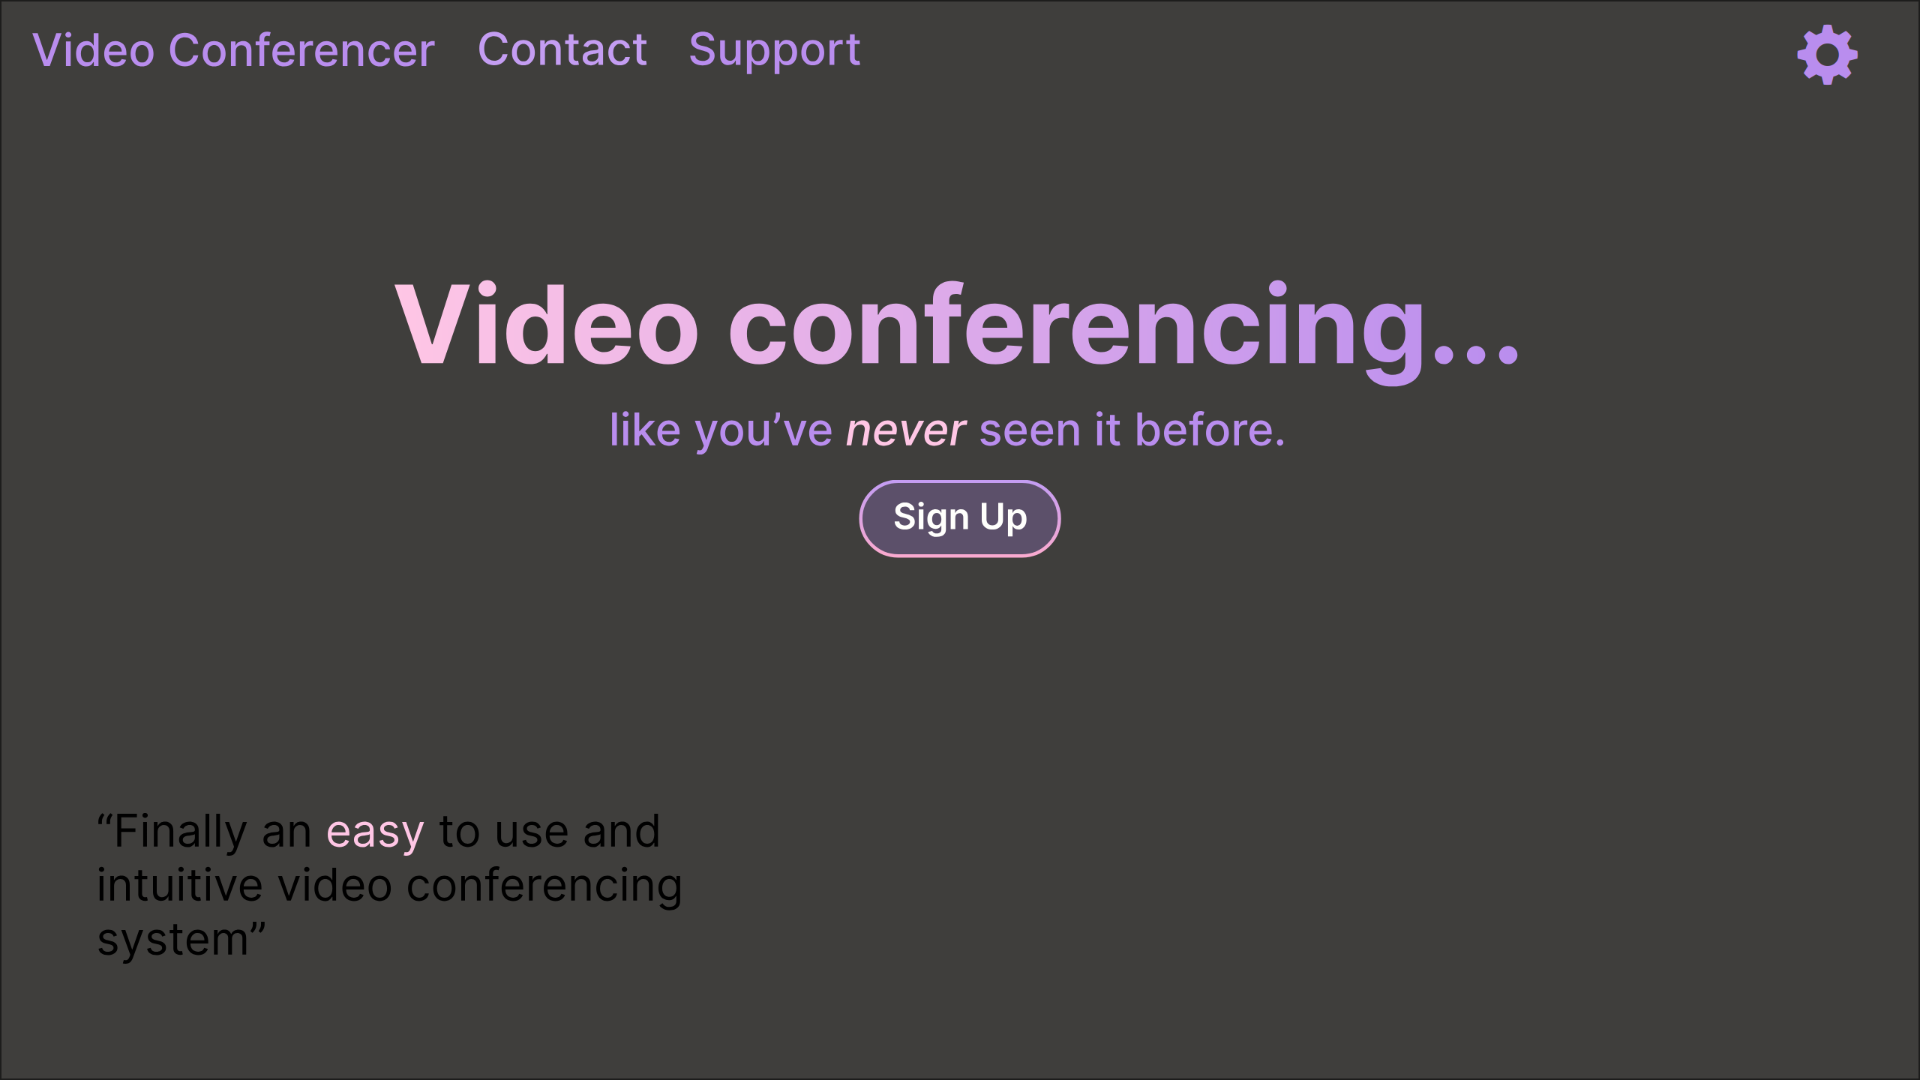
\includegraphics[scale=0.2]{Images/Proto_home3.png}

\caption{Home page prototype 3}
\end{figure}

{\color{gray} \hrulefill} \vspace{0.2cm}

{\sffamily Client feedback:}

\begin{itemize}
  \item Everything looks great!
\end{itemize}

{\color{gray} \hrulefill} 

\subsubsection{Refinements}

\textit{Description:}
I reduce the usage of vector graphics in our design,
add a gradient to the background, add a new navigation
tab and more. I conclude by cleaning up some of our CSS
code. \\ \vspace{0.2cm}

\textit{Explanation and justification:}
Not much has changed in terms of the UI of our home 
page. I added a soft gradient to out previously plain 
gray background as well as a new navigation tab "Docs".
This is where users will click in order to read the 
documentation for our back end. I added in 2 
more quotes to the bottom of the page, in a card 
format using a \texttt{.svg} graphic. I also changed 
the navbar to make use of text instead of 
\texttt{.svg} images because they are easier to align 
and will help the page load faster aswell. Then as a nice 
touch I added a simple hover transformation to the sign up 
button that makes the whole button a gradient. Finally I 
cleaned up the code and made more use of CSS's 
viewport and \texttt{margin: auto} properties, since
this would ensure that our users would have the same
UI experience no matter the size of their device. Here 
is what the refined code looks like: \\ \vspace{0.2cm}

\underline{main.html}

\begin{minted}[linenos, bgcolor=lightestgray]{html}
...
<body>
   
  <ul id="Navbar">

    <li class="Navbar_item">
      Video-Conferencer 
    </li>

    ...

    <li class="Navbar_item">
      Docs
    </li>

    <li class="Last_Navbar_item">
      <i class="glyphicon glyphicon-cog"></i>
    </li>
  </ul>

  <div id="Main">

    <object id="Headline" data="Images/Headline.svg" type="image/svg+xml">
      <img src="Images/Headline.png">
    </object>
	
    <button class="Sign_up"> <b> Sign up </b> </button> 

  </div>

  <object id="Quote" data="Images/Quote_cards.svg" type="image/svg+xml">
    <img src="Images/Quote_cards.png">
  </object>

</body>

</html>
\end{minted}

\underline{style\_main.sass}

\begin{minted}[linenos, bgcolor=lightestgray]{sass}
@import url('https://fonts.googleapis.com/css?family=Inter')
@import url('https://maxcdn.bootstrapcdn.com/bootstrap/3.3.7/css/bootstrap.min.css')

// Colour definitions
...

// Setting font and background colour
body
  height:           100vh
  margin:           0
  background-image: linear-gradient($Col_Main, $Col_Gradient)
  ... 

// Positioning the headline
#Headline
  display:      block
  margin-left:  auto
  margin-right: auto
  ...

// Styling the sign up button
.Sign_up
  border-radius:    700px
  color:            white
  background-color: $Col_Button_BG
  border:           none
  ... 

// Creates border and hover effect
.Sign_up::after
  content:          ''
  position:         absolute
  background-image: linear-gradient(to bottom, $Col_Button_Top, $Col_Button_Bot)
  z-index:          -1
  ...

.Sign_up:hover
  z-index: 0 

// Styling the navigation bar
#Navbar
  list-style-type: none
  margin:          0
  padding:         0
  ...

.Navbar_item
  color:       $Col_Secondary
  padding:     2vh
  font-size:   2.3vw
  white-space: nowrap

.Last_Navbar_item
  @extend      .Navbar_item
  margin-left: auto

// Positioning the call to action button
#Main
  display:         flex
  align-items:     center
  justify-content: center
  ...

// Positioning the quote
#Quote
  position:    fixed
  bottom:      -27px
  left:        50%
  ...
\end{minted}

This code produced this page:

\begin{figure}[H]
\centering

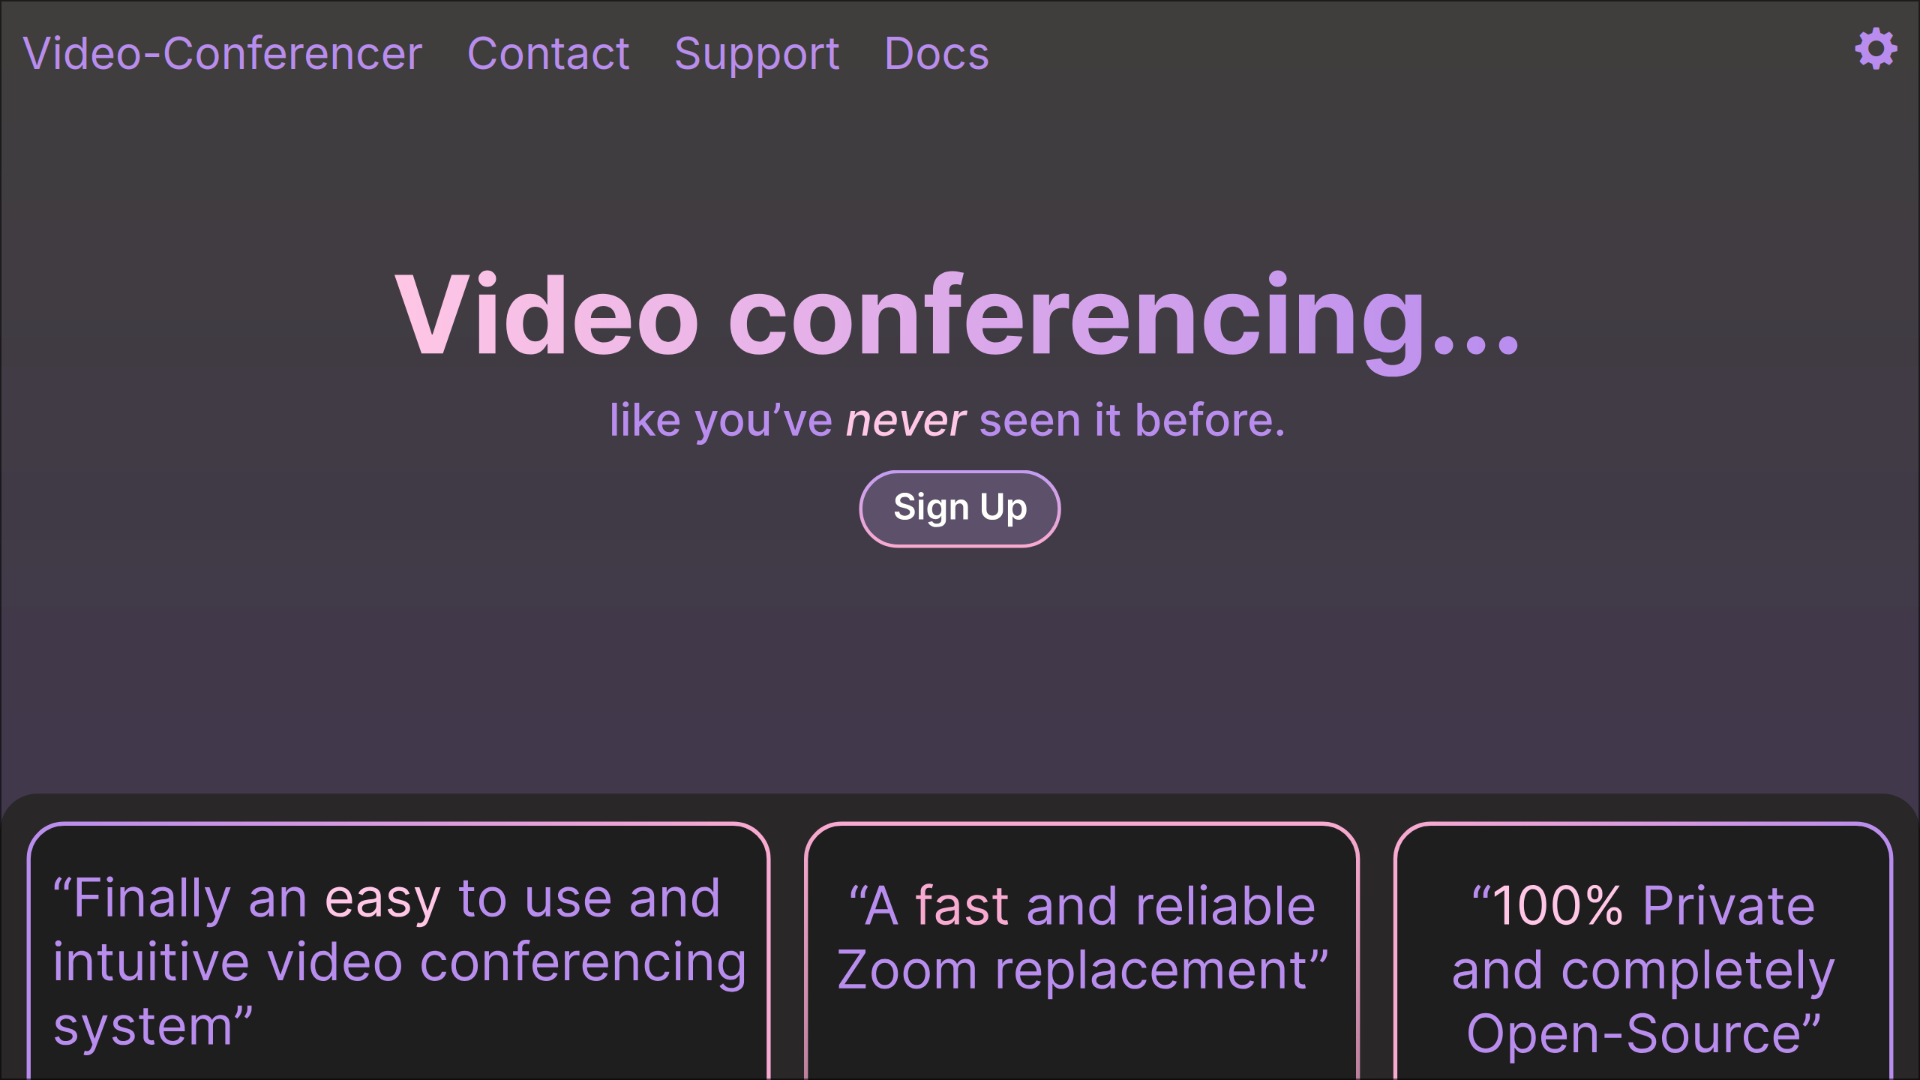
\includegraphics[scale=0.2]{Images/Refined_home.png}

\caption{Refined home page.}
\end{figure}

{\color{gray} \hrulefill} \vspace{0.2cm}

{\sffamily Development sub-task \circled{1} \faCheck}

\subsubsection{Login page}

\textit{Description:} I re-design the login page to fit with the
new theme, and implement my design in HTML and sass.\\ \vspace{0.2cm}

\textit{Explanation and justification:}
Clearly the login page needed to be re-designed also in order
to properly match the theme of the home page. Here is the 
revised design for our login page. Inspiration was drawn 
from Spline's login UI \url{https://spline.design/}.

\begin{figure}[H]
\centering

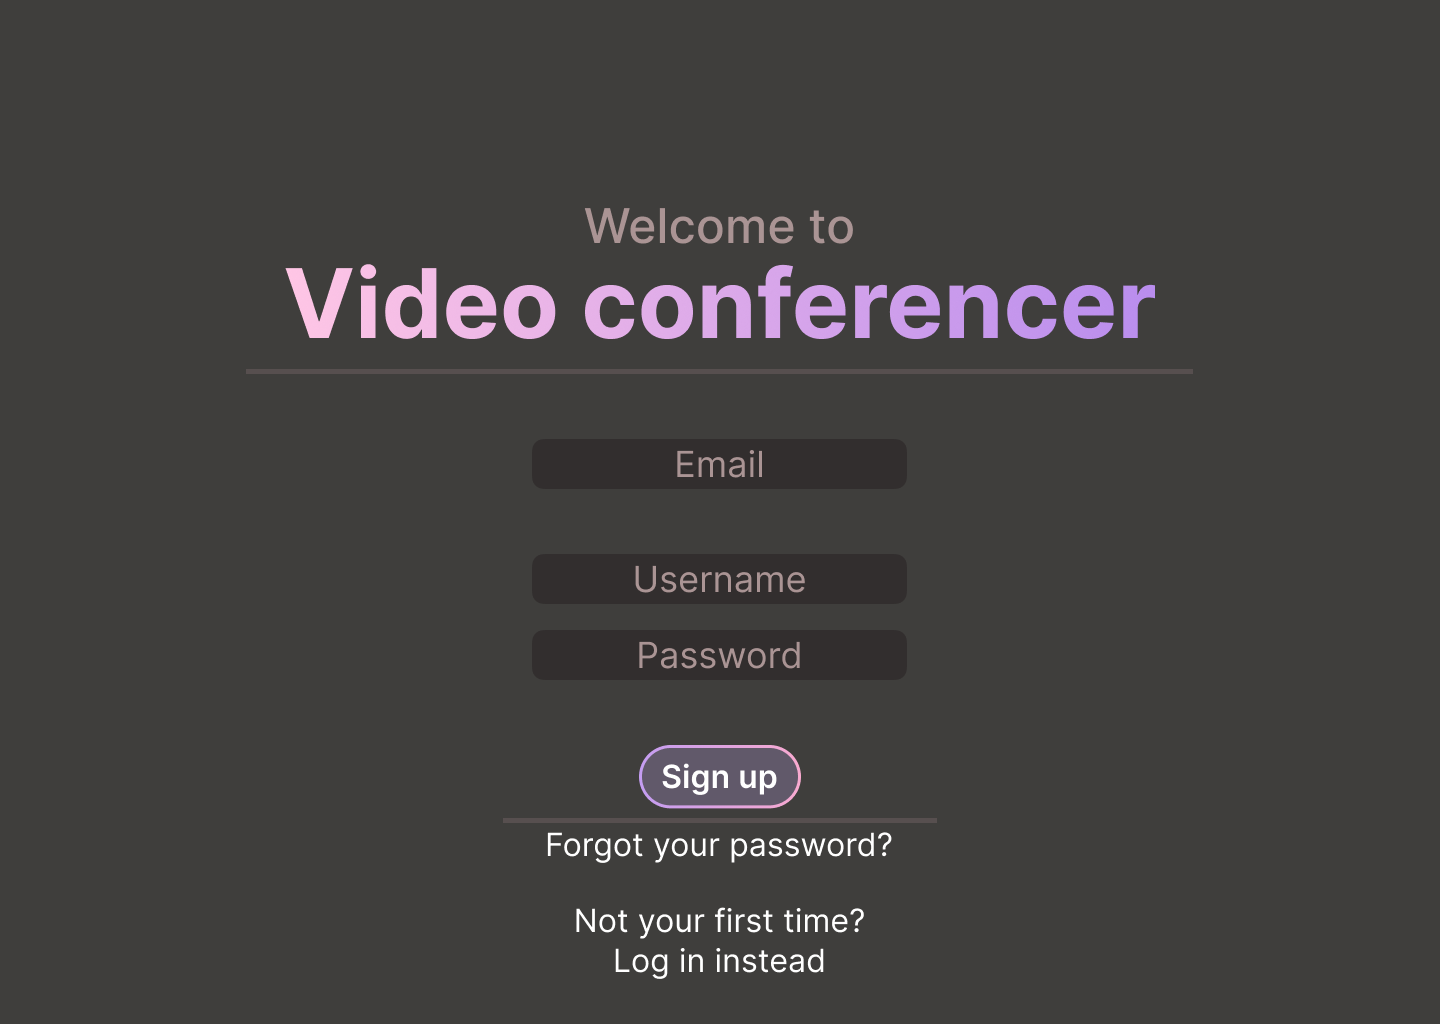
\includegraphics[scale=0.2]{Images/Login_Page_2.png}

\caption{2nd Mock up of the login page.}
\end{figure}

This revised version fits much nicer with the home page.
During the creation of this page however I realised that I 
had not yet discussed what we would do if a user had
forgotten their password. In such a case we could employ 
the standard technique of sending the user a reset password 
link to their email address and I have included this in 
our mock up. This idea will have to be added as a development
sub-task and we will tackle it's implementation in a future 
iteration. \\ \vspace{0.2cm}

The next step is to transfer the design in code, then link
our home page and login page together. During the programming
of the home page I realised that I would be using the same 
sign-up button design as the one designed on the home page.
Recalling that I would apply the DRY 
("\textbf{D}on't \textbf{r}epeat \textbf{y}ourself") principle 
whilst I wrote my code (see section \ref{sec:computational}), 
I decided to put the button code in it's own file 
\texttt{button\_styling.sass} and simply have the other \texttt{.sass}
files import from the button styling file whenever needed. Now
that I had gained some experience with translating my designs into 
HTML and CSS I was able to make some changes to the design on the 
fly to improve upon the figma mock up design. \\ \vspace{0.2cm}

\underline{login.html}

\begin{minted}[linenos, bgcolor=lightestgray]{html}
...
<body>

  <object id="Headline" data="Images/Welcome.svg" type="image/svg+xml">
    <img src="Images/Welcome.png">
  </object>

  <center>
    <b id="Login_Prompt"> Log in instead? Click here </b> 
  </center>

  <br><br>

  <center>

    <div id="Login">

      <form>
	<input type="text" placeholder="Email" name="email" required>       <br><br><br>
	<input type="text" placeholder="Username" name="username" required> <br><br>
	<input type="password" placeholder="Password" name="password" required autofocus> 
	<br> <br> <br>

	<button class="Button"> <b> Sign up </b> </button> <br><br>

	<div class="Rule"> </div> <br>

	<p style="color:white; font-size: 20px"> Forgot your password? </p>
      </form>
    ...
\end{minted}

\underline{styles\_login.sass}

\begin{minted}[linenos, bgcolor=lightestgray]{sass}
@use './button_styling.sass'
@import url('https://fonts.googleapis.com/css?family=Inter')
@import url('https://maxcdn.bootstrapcdn.com/bootstrap/3.3.7/css/bootstrap.min.css')

// Colour definitions
...

// Setting font and background colour
body
  height:           100vh
  margin:           0
  background-color: $Col_Main
  ...

.Rule
  width: 40%
  border-bottom: 4px solid $Col_Rule

// Positioning the headline
#Headline
  display:      block
  margin-left:  auto
  margin-right: auto
  ... 

// Positioning the login box
#Login
  disply:       block
  margin-left:  auto
  margin-right: auto

// Styling the input field
input 
  border-radius:    12px
  width:            281px
  height:           37.5px
  ...

#Login_Prompt
  color:     white
  font-size: 20px
\end{minted}

This code produced our first prototype:

\begin{figure}[H]
  \centering
  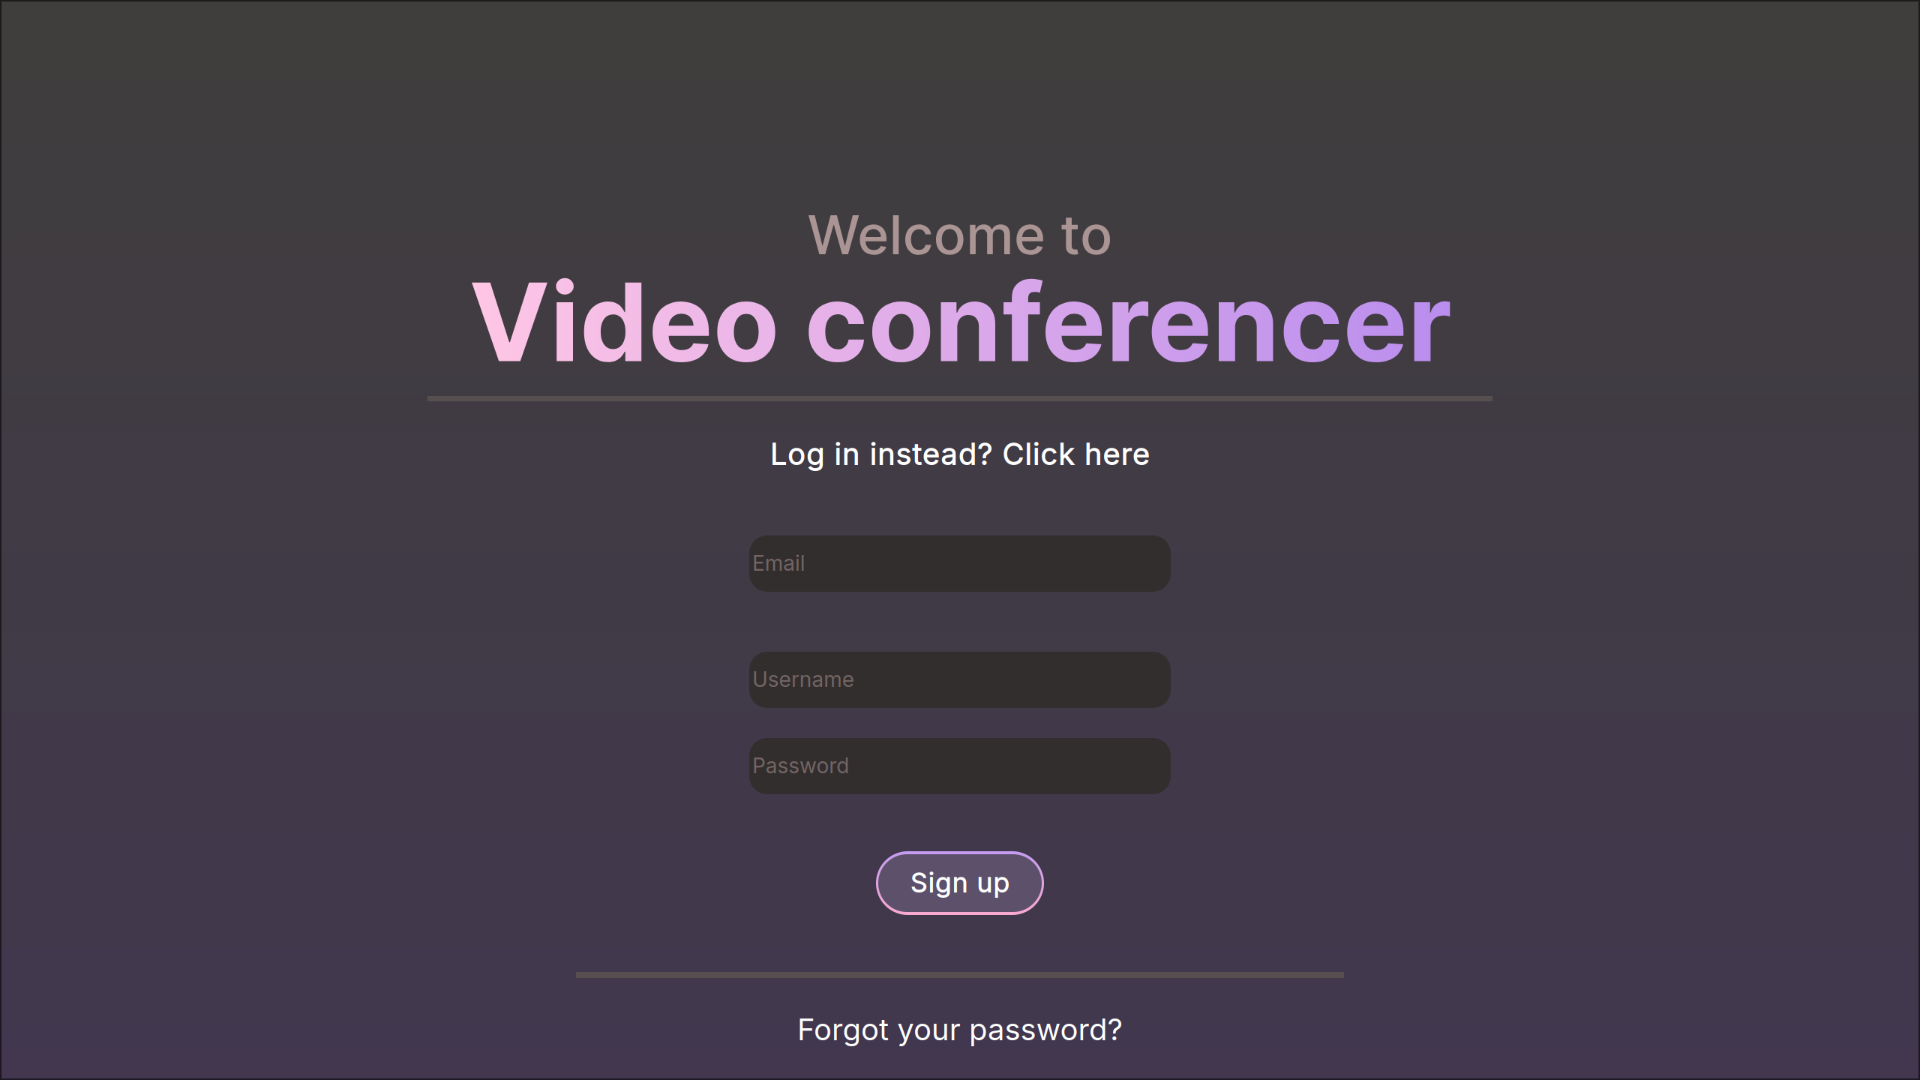
\includegraphics[scale=0.2]{Images/LoginUI.png}
  \caption{Login UI prototype 1}
\end{figure}

{\color{gray} \hrulefill} \\ \vspace{0.2cm}

{\sffamily Client feedback:}

\begin{itemize}
  \item Looks great!
\end{itemize}

{\color{gray} \hrulefill}
\vspace{0.2cm}

{\sffamily Development sub-task \circled{1.2} \faCheck} \\
\vspace{0.2cm}

The current file structure of our project is as follows: \\
\vspace{0.2cm}

\begin{forest}
  pic dir tree,
  where level=0{}{
    directory,
  },
[src
  [Images]
  [main.html, file]
  [login.html, file]
  [styles\_main.sass, file]
  [styles\_login.sass, file]
  [styles\_main.css, file]
  [styles\_login.css, file]
  [button\_styling.sass, file]
] 
\end{forest}

\vspace{0.3cm}
Look at Github commit
\texttt{54e06ac60f0876086c259f29ce23eae89ff4aad6} to 
see the state of the project after our first iteration.\\
\vspace{0.1cm}

Alternatively click the following link to view the state of 
the project at this point in development: \\ 
\href{https://github.com/zzzNathan/Video-Conferencer/tree/54e06ac60f0876086c259f29ce23eae89ff4aad6}{
\texttt{VideoConferencer-Iteration1}}.

\section{Iteration 2}

During this iteration I wanted to design and implement
some of the underlying infastructure behind our application
and complete development subtasks \circled{2} and \circled{A}.\\
\vspace{0.2cm}

\textit{Description:}
After doing some of research into free web deployment 
services I settled on using Vercel in order to deploy my website.\\
\vspace{0.2cm}

\textit{Explanation and justification:}
Here are a few of the other options I looked into and why I rejected
them. \\ \vspace{0.2cm}

\begin{tblr}{colspec={XX}, row{1}={lightestgray}}
Service & Explanation \\

Railway.app & You can only use \$5.00 worth of resources on the
free tier, once this is depleted the project won't be up 
anymore \\

render.com & Projects on the free tier are deleted automatically after 1 month \\
\end{tblr}

On the other hand Vercel doesn't have any of these drawbacks, so my 
site will be able to stay up permanently so long as some resource limits are
not crossed. \\ \vspace{0.2cm}

\textit{Description:} In order to use Vercel to deploy my web
application I had to use a web framework. I chose to use React with 
Vite and rewrote my existing codebase to work with this framework. \\ 
\vspace{0.2cm}

\textit{Explanation and justification:}
Initially I intended to try and stay away from all of these
web-frameworks and just stick to plain old HTML and CSS (or 
sass in our case), however an issue arose when I wanted to 
redirect users to our registration page once they clicked 
the sign up button on our home page. For whatever reason 
the redirection would work when I hosted the application on 
my own machine, however when I would deploy to vercel the 
redirection would either, simply not change page or display
a 404 code not found error.

\begin{figure}[h]
\centering

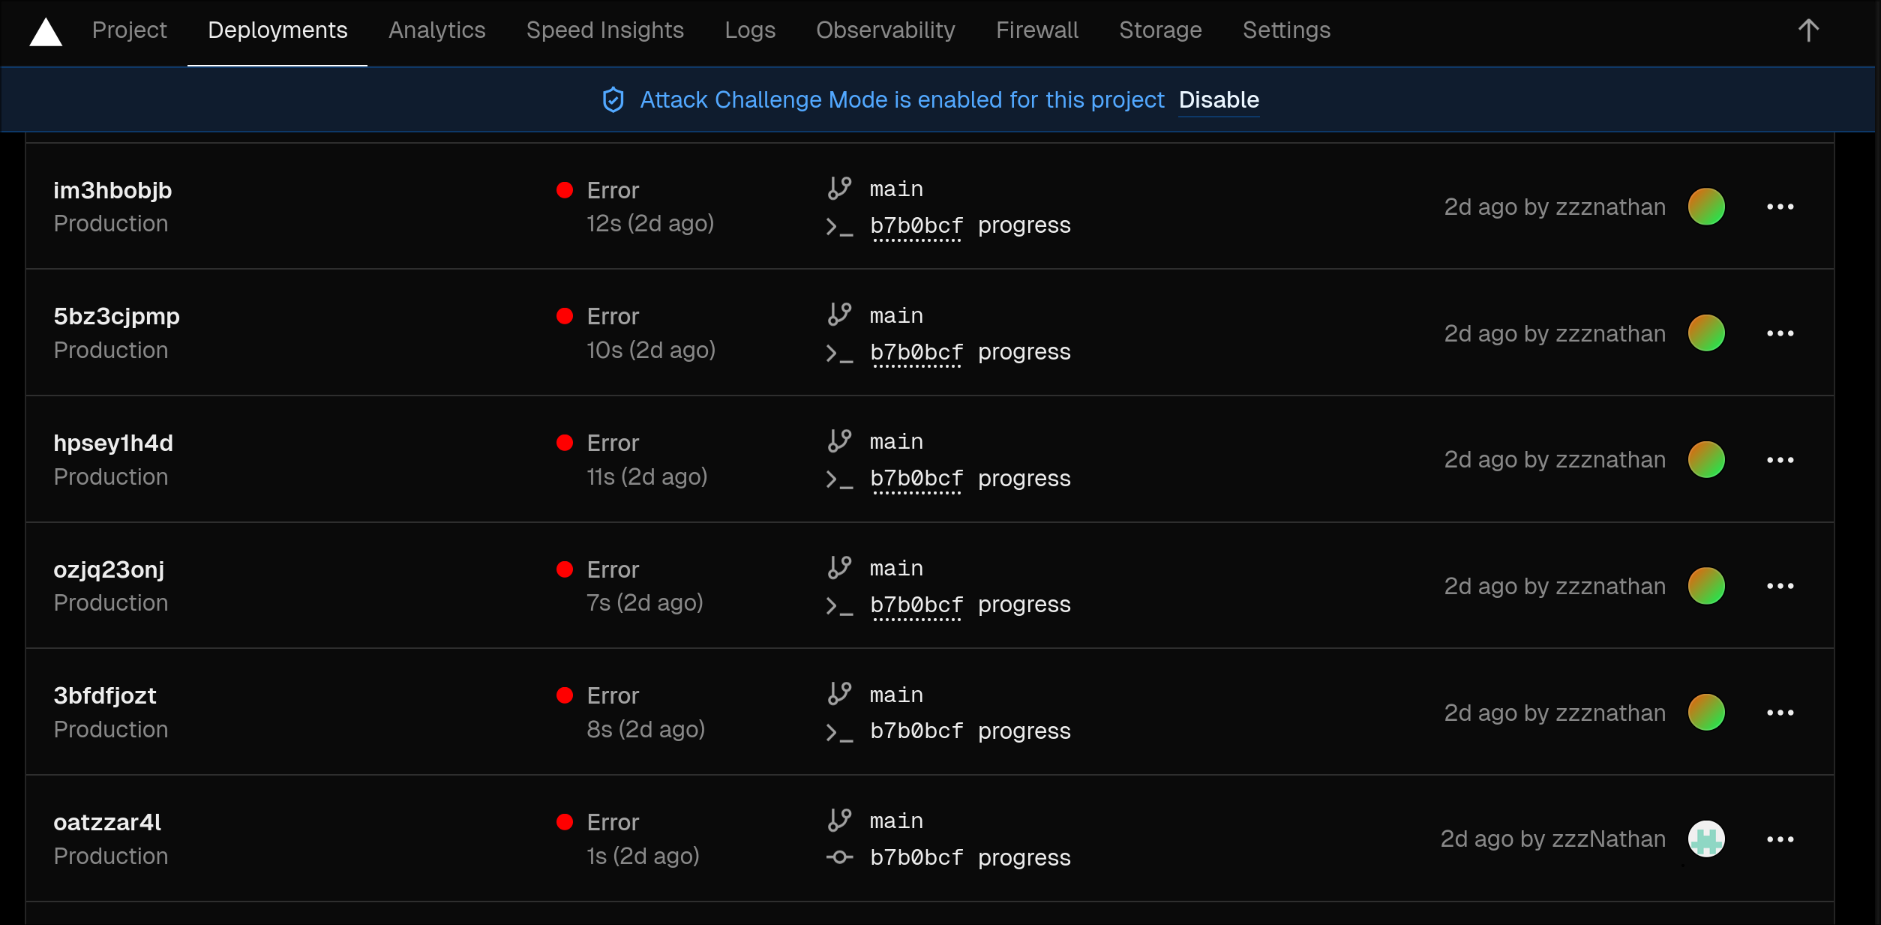
\includegraphics[scale=0.2]{Images/Vercel_Errors.png}

\caption{Errors when deploying to Vercel.}

\end{figure}

Eventually after a lot of trial and error and some research,
I found out that using a router with react would allow us to
redirect the user to different pages once deployed. I then 
took some time to migrate our codebase to JSX to work with the
react framework. We will omit the code for the re-written
webpages since it is pretty similar to the snippets shown in 
Iteration 1. Here is what the routing logic looks like. \\
\vspace{0.2cm}

\underline{main.jsx} \\ \vspace{0.2cm}

\begin{minted}[linenos, bgcolor=lightestgray]{jsx}
import { createRoot } from "react-dom/client"
import { createBrowserRouter, RouterProvider } from "react-router-dom"
import Home from "./components/Home.jsx"
import Registration from "./components/Registration.jsx"

// Path is an extension that goes after our URL,
// once this extension is written the corresponding
// React element will be loaded and rendered.
const router = createBrowserRouter([
  {
    path: "/",
    element: <Home />
  },
  {
    path: "/registration",
    element: <Registration />
  }
])

createRoot(document.getElementById('root')).render(
  <RouterProvider router={router} />
)
\end{minted}

\textit{Description:} I used the Clerk user management
platform to create a user account registration form.\\
\vspace{0.2cm}

\textit{Explanation and justification:} I originally wanted to 
do this task manually, creating my own table and then querying
this table in order to add new users and log users in. However
after doing some reading and looking over Stack Overflow posts 
like this one \url{https://stackoverflow.com/questions/46819734/how-to-check-username-and-password-matches-the-database-values}
I realised that many issues can arise when developers try to 
implement these systems themselves. In order to avoid this 
plethora of issues I instead chose to use the Clerk.com API 
\footnote{I originally came across this API watching Theo T3.gg's 
React tutorial.}
for user authentication. Not only was it much easier to implement
but the usage of this API also ensures that I wont have to worry
about any security issues, since the API has been thoroughly
tested. Here's the implementation. \\ \vspace{0.2cm}

\underline{Registration.jsx}
\begin{minted}[linenos, bgcolor=lightestgray]{jsx}
import { ReactTyped } from "react-typed"
import { ClerkProvider, SignedOut, SignUp } from "@clerk/clerk-react"
import { dark } from "@clerk/themes"
import Navbar from "./Navbar" 
import "../styles/Registration.sass"

const PUBLISHABLE_KEY = import.meta.env.VITE_CLERK_PUBLISHABLE_KEY
...

function Registration () {
  return (
  <> <Navbar />
    <Headline />
    
    <ClerkProvider publishableKey={PUBLISHABLE_KEY}>
      <SignedOut>
        <center> <SignUp appearance={dark}/> </center>
      </SignedOut>
    </ClerkProvider>
  </>
  )
}

export default Registration
\end{minted}

{\color{gray} \hrulefill}
\vspace{0.2cm}

{\sffamily Tests}
\begin{itemize}
  \item Site home page loads correctly \faCheck \\
  \item Correctly redirected to registration page \faCheck \\
  \item Users can create a new account \faCheck \\
\end{itemize}

{\color{gray} \hrulefill}
\vspace{0.2cm}

You can try these features out yourself at \url{https://video-conferencer.vercel.app/registration}.
(May not work if development is ongoing).\\ \vspace{0.2cm}

{\sffamily Development sub-task \circled{2} \faCheck \\ \vspace{0.2cm}
Development sub-task \circled{A} \faCheck }

The current file structure of our project is as follows: (
Ignoring configuration files)
\\ \vspace{0.2cm}

\begin{forest}
  pic dir tree,
  where level=0{}{
    directory,
  },
[Video-Conferncer
  [index.html, file],
  [src
    [main.jsx, file]
    [assets
      [Quote\_Cards.svg, file]
    ],
    [components
      [Button.jsx, file],
      [Home.jsx, file],
      [Navbar.jsx, file],
      [Registration.jsx, file]
    ],
    [styles
      [Button.sass, file],
      [Home.sass, file],
      [Navbar.sass, file],
      [Registration.sass, file]
    ]
  ]
] 
\end{forest}
\vspace{0.3cm}
